\documentclass{article}
\usepackage{booktabs}
\usepackage{array}
\usepackage{tikz}
\usepackage[table]{xcolor} % for \cellcolor

\begin{document}

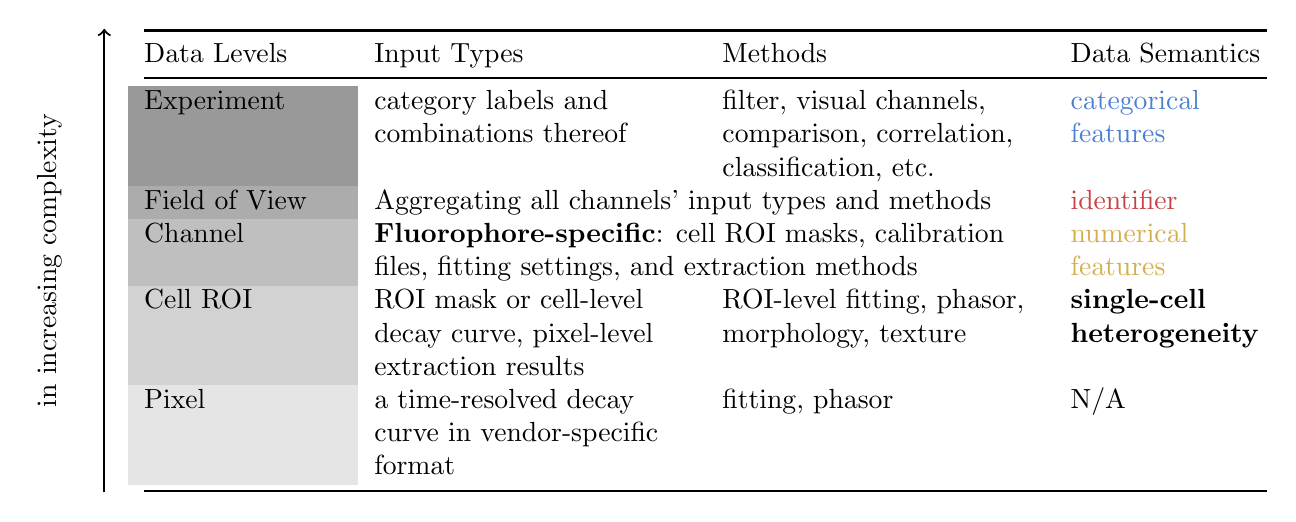
\begin{tikzpicture}
\node[inner sep=0] (tbl) {%
\begin{tabular}{@{} >{\raggedright\arraybackslash}p{2.5cm}
                    >{\raggedright\arraybackslash}p{4cm}
                    >{\raggedright\arraybackslash}p{4cm}
                    >{\raggedright\arraybackslash}p{2.5cm} @{}}
  \toprule
  Data Levels & Input Types & Methods & Data Semantics \\
  \midrule
  \cellcolor{gray!80}Experiment
    & category labels and combinations thereof
    & filter, visual channels, comparison, correlation, classification, etc.
    & \textcolor[HTML]{4880D4}{categorical features}\\
  \cellcolor{gray!65}Field of View
    & \multicolumn{2}{>{\raggedright\arraybackslash}p{8cm}}{Aggregating all channels' input types and methods}
    & \textcolor[HTML]{C94146}{identifier} \\
  \cellcolor{gray!50}Channel
    & \multicolumn{2}{>{\raggedright\arraybackslash}p{8cm}}{%
        \textbf{Fluorophore-specific}: cell ROI masks, calibration files, fitting settings,
        and extraction methods}
    & \textcolor[HTML]{D3AE4A}{numerical features} \\
  \cellcolor{gray!35}Cell ROI
    & ROI mask or cell-level decay curve, pixel-level extraction results
    & ROI-level fitting, phasor, morphology, texture
    & \textbf{single-cell heterogeneity} \\
  \cellcolor{gray!20}Pixel
    & a time-resolved decay curve in vendor-specific format
    & fitting, phasor
    & N/A \\
  \bottomrule
\end{tabular}%
};

% Left-side arrow from top to bottom
\draw[->,thick]
  ([xshift=-5mm]tbl.south west) -- ([xshift=-5mm]tbl.north west)
  node[midway,xshift=-7mm,rotate=90,align=center]
  {in increasing complexity};

\end{tikzpicture}

\end{document}
